\begin{center}
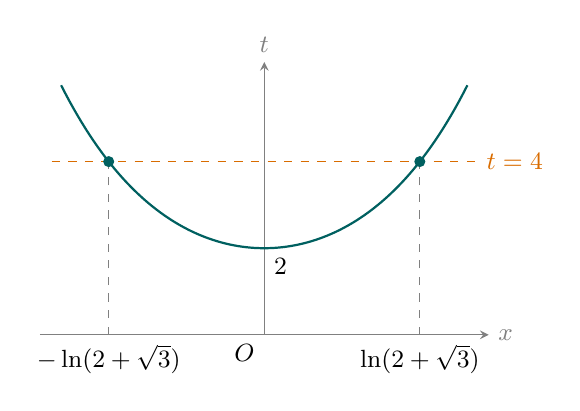
\begin{tikzpicture}[x=1.5cm,y=0.55cm,>=stealth,font=\small]
\draw[->,gray] (-1.9,0)--(1.9,0) node[right] {$x$};
\draw[->,gray] (0,0)--(0,6.3) node[above] {$t$};
\draw[teal!75!black,thick,domain=-1.72:1.72,samples=100] plot (\x,{exp(\x)+exp(-\x)});
\draw[orange!85!black,dashed] (-1.8,4)--(1.8,4) node[right] {$t=4$};
\draw[dashed,gray] (-1.31696,0)--(-1.31696,4) (1.31696,0)--(1.31696,4);
\fill[teal!75!black] (-1.31696,4) circle (2pt) (1.31696,4) circle (2pt);
\node[below] at (-1.31696,0) {$-\ln(2+\sqrt3)$};
\node[below] at (1.31696,0) {$\ln(2+\sqrt3)$};
\node[below left] at (0,0) {$O$};
\node[below right] at (0,2) {$2$};
\end{tikzpicture}
\end{center}
